% begin module natural-logarithm-def-ex8
\begin{frame}
\begin{example}%[Example 8, p. 408]
Draw the graph of $y = \ln (x - 2) -1$.
\ \only<handout:0| -1>{%
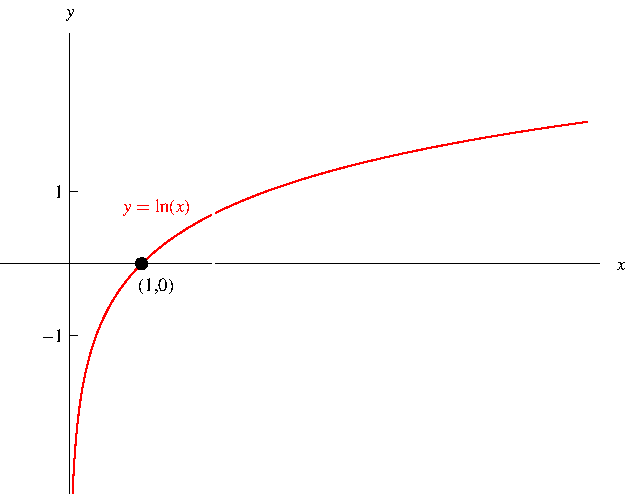
\includegraphics[height=6cm]{logarithms/pictures/07-03-ex8a.pdf}%
}%
\only<handout:0| 2>{%
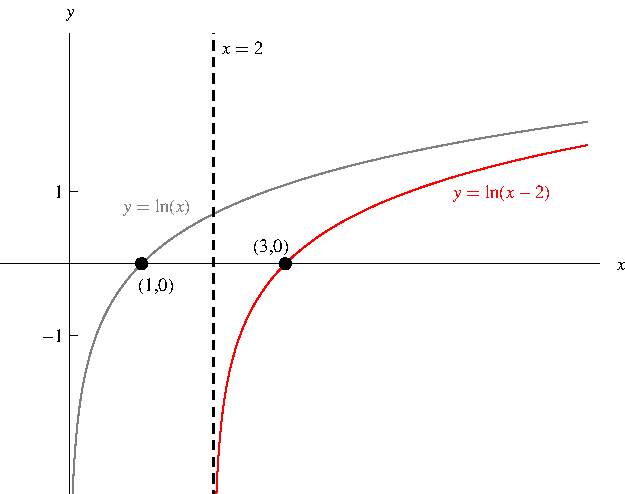
\includegraphics[height=6cm]{logarithms/pictures/07-03-ex8b.pdf}%
}%
\only<3->{%
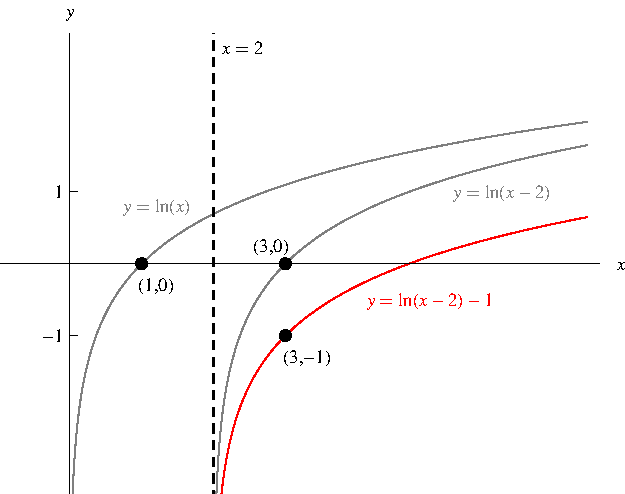
\includegraphics[height=6cm]{logarithms/pictures/07-03-ex8c.pdf}%
}%
\end{example}
\end{frame}
% end module natural-logarithm-def-ex8
